\documentclass[10pt]{beamer}
\usepackage[slovak]{babel}
\usepackage[IL2]{fontenc}
\usepackage[utf8]{inputenc}
\usepackage{graphicx}
\usepackage{utopia} %font utopia imported
\usetheme{CambridgeUS}
\usepackage{booktabs}
\usepackage{url} 
\usepackage{hyperref} 
\usepackage{booktabs}



\usecolortheme{dolphin}

% set colors
\definecolor{myNewColorA}{RGB}{126,12,110}
\definecolor{myNewColorB}{RGB}{165,85,154}
\definecolor{myNewColorC}{RGB}{203,158,197}
\setbeamercolor*{palette primary}{bg=myNewColorC}
\setbeamercolor*{palette secondary}{bg=myNewColorB, fg = white}
\setbeamercolor*{palette tertiary}{bg=myNewColorA, fg = white}
\setbeamercolor*{titlelike}{fg=myNewColorA}
\setbeamercolor*{title}{bg=myNewColorA, fg = white}
\setbeamercolor*{item}{fg=myNewColorA}
\setbeamercolor*{caption name}{fg=myNewColorA}
\usefonttheme{professionalfonts}
\usepackage{natbib}
\usepackage{hyperref}
%------------------------------------------------------------

\setbeamerfont{title}{size=\large}
\setbeamerfont{subtitle}{size=\small}
\setbeamerfont{author}{size=\small}
\setbeamerfont{date}{size=\small}
\setbeamerfont{institute}{size=\small}
\title[FIIT STU]{Gamifikácia a seriózne hry v medicínskom vzdelávaní}
\author[Petra Miková]{Petra Miková}

\institute[]{ Semestrálny projekt v predmete Metódy inžinierskej práce, ak. rok 2022/23, vedenie: Ing. Ladislav Zemko}
\date[ 25. november 2022]
{25. november 2022}

%------------------------------------------------------------
%This block of commands puts the table of contents at the 
%beginning of each section and highlights the current section:
%\AtBeginSection[]
%{
%  \begin{frame}
%    \frametitle{Contents}
%    \tableofcontents[currentsection]
%  \end{frame}
%}


\begin{document}

%The next statement creates the title page.
\frame{\titlepage}
\begin{frame}
\frametitle{Obsah}
\tableofcontents
\end{frame}
%------------------------------------------------------------
\section{Úvod}
    \begin{frame}{Úvod}
 \begin{itemize}
  \setlength\itemsep{2em}
\item v medicíne je efektívne memorovanie učiva dôležitejšie než kdekoľvek inde
	\begin{itemize}
	\item vieme tomu dopomôcť gamifikáciou
	\end{itemize}
	
\item pre vykonávanie povolania lekára je dôležitá praktická výučba
	\begin{itemize}
	\item vo veľa prípadoch je však počas štúdia nedostatočná
	\item v tomto vie vo veľkej miere pomôcť VR v serióznych hrách
	\end{itemize}

\end{itemize}
    \end{frame}
    
\section{Gamifikácia v medicínskom vzdelávaní}\label{gamifikacia}
    \begin{frame}{Gamifikácia v medicínskom vzdelávaní}
  \begin{itemize}
  \setlength\itemsep{2em}
\item gamifikácia využíva aplikáciu hernej mechaniky, estetiky a herného myslenia na motiváciu k činnosti
	\begin{itemize}
	\setlength\itemsep{1em}
	\item skóre, odznaky za splnené ciele, či časové obmedzenia na naučenie sa daného učiva
	\end{itemize}
	
\item odosielanie notifikácii - "spaced repetition"
	\begin{itemize}
	\item opakovanie učiva efektívnou formou
	\end{itemize}
	
\item bodovací systém v aplikácii
	\begin{itemize}
	\item sledovanie pokroku
	\item vytvorenie rebríčka
	\end{itemize}

\end{itemize}
    \end{frame}
    
\subsection{Prototyp aplikácie}\label{gamifikacia:aplikacia}
    \begin{frame}{Prototyp aplikácie}
      \begin{itemize}
  \setlength\itemsep{2em}
\item medik v aplikácii vidí jemu prístupné levely, ktoré si odomýka neskôr práve zbieraním bodov v testoch z predošlých levelov
	
\item v každom leveli je sprístupnený materiál s 3D vizualizáciou a prichystané testy
	
\item absolvovanie prvého testu
	\begin{itemize}
	\item sprístupnenie materiálu sústrediaceho sa práve na učivo v ktorom počas pretestovania medik urobil chybu
	\end{itemize}
	
\item notifikácia k opätovnému zopakovaniu materiálu

\item finálny test
	\begin{itemize}
	\item body ktoré medik využije na sprístupnenie ďalšieho levelu
	\item zostavenie rebríčka
	\end{itemize}

\end{itemize}
\end{frame}

\subsection{Diagram funkcionalít aplikácie}\label{gamifikacia:diagram}
    \begin{frame}{Diagram funkcionalít aplikácie}
     
\begin{figure}[tbh]
\centering
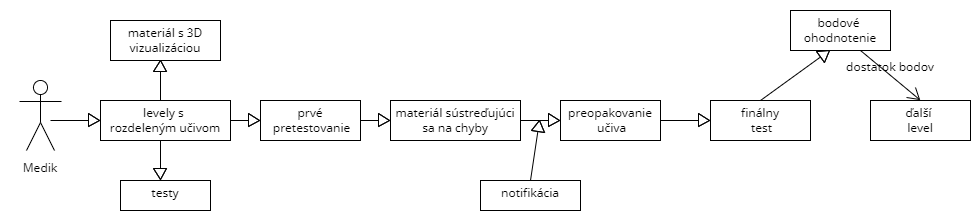
\includegraphics[scale=0.35]{dia.png}
\caption{Diagram zobrazujúci funkcionality aplikácie pre učenie medikov.}
\label{diagram}
\end{figure}

\end{frame}
    
\section{Prax medikov a seriózne hry}
    \begin{frame}{Prax medikov a seriózne hry}
  \begin{itemize}
  \setlength\itemsep{2em}
\item praktická výučby medicíny prebieha najmä na kadávroch, a v neskoršom štádiu štúdia aj na reálnych pacientoch
	\begin{itemize}
	\item kadávrov je vo všeobecnosti nedostatok
	\item výučba operačných úkonov na reálnych pacientoch je nie vždy bezpečná
	\end{itemize}
	
\item je efektívnejšie pristúpiť na výučbu, najmä anatómie, pomocou virtuálnej reality
	\begin{itemize}
	\item umožňuje využívať 3D priestor na pochopenie priestorových vzťahov medzi časťami tela
	\item s týmito časťami je možné interagovať a manipulovať práve v prostredí virtuálnej reality za pomoci dostupných periférií
	\end{itemize}
	
\item simulovaný tréning operačných úkonov za pomoci virtuálnej reality
	\begin{itemize}
	\item simulátor umožňuje tréning bez nátlaku a opakovanie úkonov toľkokrát, koľko je pre daného medika potrebné

	\end{itemize}
\end{itemize}
    \end{frame}

\section{Prieskum}\label{prieskum}
    \begin{frame}{Prieskum}
  \begin{itemize}
  \setlength\itemsep{1.3em}
\item prieskum medzi študentami medicíny o tom, čo si myslia o implementovaní častí informatiky do výučby medicíny
	\begin{itemize}
	\item dotazník pozostával z troch otázok
	\item prieskumu sa zúčastnilo 56 respondentov
	\end{itemize}
	
\item prvá otázka: "Bol by pre vás pri učení sa anatómie prínosný VR headset, vďaka ktorému by ste si v reálnom čase vedeli prezerať časti tela v 3D priestore a z viacerých uhlov?"
	\begin{itemize}
	\item áno: 52 medikov, nie: 4 medici
	\end{itemize}
	
\item druhá otázka: "Cítili by ste sa pri vykonávaní prvej operácie sebavedomejšie, ak by ste ju mali odskúšanú vo forme realistickej hry využívajúcej virtuálnu realitu?"
	\begin{itemize}
	\item áno: 51 medikov, nie: 5 medici
	\end{itemize}
	
\item tretia otázka: "Motivovalo by vás učiť sa viac, ak by ste vedeli v aplikácii na učenie sa svoje dosiahnuté skóre a čas strávený učením porovnať s ostatnými študentami v ročníku?"
	\begin{itemize}
	\item áno: 28 medikov, nie: 28 medikov
	\end{itemize}
	
\end{itemize}
\end{frame}


\subsection{Tabuľka ku prieskumu}\label{prieskum:tabulka}
    \begin{frame}{Tabuľka ku prieskumu}
\begin{table}[hbtp]
\centering
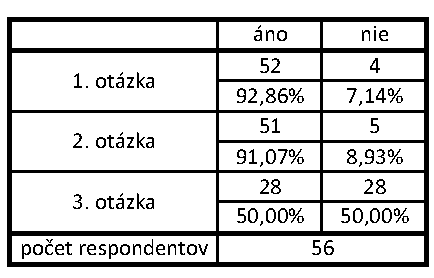
\includegraphics[scale=0.9]{tabulkakprojektu.pdf}
\caption{Tabuľka ku vykonanému prieskumu.}
\end{table}
    
    \end{frame}


\section{Záver}
    \begin{frame}{Záver}
    \begin{itemize}
  \setlength\itemsep{2em}
\item pomocou gamifikácie a serióznych hier vieme výrazne zefektívniť výučbu medicíny

\item ukázali sme si návrh aplikácie pre učenie sa medikov s použitím gamifikácie

\item virtuálna realita vie vo veľkej miere ovplyvniť nie len efektivitu, ale aj bezpečnosť praktickej výučby

	
\item podľa prieskumu sú aj samotní medici za implementáciu informatiky do ich vzdelávania
	
\item prieskum ukázal aj to, že motivácia vo forme bodového ohodnotenia a následneho porovnania s ostatnými nie je pre každého


\end{itemize}
    \end{frame}
    


\section*{Acknowledgement}  
\begin{frame}
\textcolor{myNewColorA}{\Huge{\centerline{Ďakujem za pozornosť!}}}
\end{frame}

\end{document}



